\documentclass[a4paper,12pt]{article}
\usepackage[utf8]{inputenc}
\usepackage[spanish]{babel}
\usepackage{hyperref}
\usepackage{geometry}
\usepackage{graphicx}

% Configuración de márgenes
\geometry{left=2.5cm,right=2.5cm,top=3cm,bottom=3cm}

% Configuración del enlace clicable
\hypersetup{
    colorlinks=true,
    linkcolor=blue,
    urlcolor=blue,
    pdftitle={Implementación del Juego 3 en Raya},
    pdfauthor={Adrián Martínez Pérez, Guillem Arnau Vallejos}
}

% Información del documento
\title{Implementación del Juego 3 en Raya}
\author{Adrián Martínez Pérez \\ Guillem Arnau Vallejos}
\date{Facultad de Informática de Barcelona \\ Grado de Inteligencia Artificial}

\begin{document}

\maketitle
\tableofcontents
\newpage

\section{Introducción}
El objetivo de esta práctica es implementar un tablero abstracto para el juego 3 en raya, utilizando el módulo
\texttt{pygame} de \texttt{python3}. Inicialmente, en esta primera versión, hemos desarrollado el juego para ser
 jugado por dos personas, en lugar de incluir una inteligencia artificial que permita competir contra la máquina,
 decisión la cual nos ha permitido enfocarnos en el desarrollo de la lógica del juego y en la creación de una buena 
 experiencia de usuario funcional y accesible.

 \vspace{\baselineskip}
 También hemos hecho accesible el código para todo aquel que quiera leerlo, entenderlo o modificarlo, ya que está todo
 comentado en la medida de lo posible, tanto lo que hacen las funciones, como las diferentes partes de ellas. 
 Además, todo el juego ha sido desarrollado para que pueda ser cambiado el tamaño del teablero y las piedras por jugador,
 simplemente cambiando el valor de \texttt{BSIZ} y \texttt{ST\_PLAYER} en el archivo \texttt{constants.py}, manteniendo una 
 dinámica más entretenida se pretende jugar con un tablero más grande para hacer el juego más largo (y más complicado).

 \vspace{\baselineskip}
 El juego consta de cinco archivos principales que estructuran el código 
 y separan las funcionalidades esenciales:

 \begin{itemize}
    \item \textbf{\texttt{abs\_board\_h.py}}: Funciones y lógica necesarias para gestionar el estado del tablero,
    verificar condiciones de victoria y manejar los movimientos de los jugadores.
    \item \textbf{\texttt{constants.py}}: Este archivo sirve para almacenar todas las constantes necesarias para el
    funcionamiento del programa.
    \item \textbf{\texttt{utils.py}}: Implementa las utilidades del juego: tanto las pantallas de carga en el modo texto
    (\texttt{txt}) como en la interfaz gráfica (\texttt{gui}), y el menú principal.
    \item \textbf{\texttt{main\_gui.py}}: Implementa la interfaz gráfica de usuario. Contiene la configuración inicial,
    creación de ventanas e integración con \texttt{abs\_board\_h.py}.
    \item \textbf{\texttt{main\_txt.py}}: Implementa la versión para consola del juego, con colores y mejoras visuales
    para un mayor atractivo.
\end{itemize}

En la carpeta de la práctica se incluye todo lo necesario para la ejecución y disfrute del juego. Solo es necesario
ejecutar dos archivos para jugar al juego:

\begin{itemize}
    \item Para jugar en modo texto, ejecutar en la consola el siguiente comando:
    \begin{verbatim}
    $ python3 main_txt.py
    \end{verbatim}
    \item Para jugar en modo gráfico, ejecutar en la consola el siguiente comando:
    \begin{verbatim}
    $ python3 main_gui.py
    \end{verbatim}
\end{itemize}

\section{Metodología de la Implementación}
El desarrollo de este proyecto ha sido un trabajo colaborativo entre Adrián Martínez Pérez y Guillem Arnau Vallejos,
mediante un repositorio compartido en la plataforma \texttt{GitHub}. Esta plataforma nos permitió realizar un seguimiento
de los cambios, revertir errores y garantizar la estabilidad del código en cada etapa del desarrollo. GitHub ha sido una 
excelente plataforma para la colaboración en este tipo de proyectos, y hemos disfrutado mucho aprendiendo a utilizarla.

\vspace{\baselineskip}
En cuanto a la distribución de tareas, adoptamos un enfoque flexible. No dividimos las tareas de manera estricta, sino que
trabajamos de forma iterativa comunicándonos constantemente sobre los avances, problemas encontrados, mejoras implementadas y 
las ideas para futuras versiones. Esta dinámica fomentó un ambiente de aprendizaje mutuo y creatividad.

\vspace{\baselineskip}
Para la implementación de este código, hemos añadido un archivo que no estaba originalmente: \texttt{utils.py}, y hemos
modificado todos los archivos con el fin de lograr una buena implementación, teniendo creatividad además de añadir nuevas
funciones y utilidades, como una animación de carga para el modo de juego txt.

\section{Modos de juego}
El 3 en raya moderno ganó popularidad en Europa tras la Edad Media, todo debido a su simplicidad, y además, se podía jugar facilmente
con materiales rudimentarios, como piedras (de ahí viene el nombre original de las fichas), y un tablero dibujado en la tierra. Este juego 
ha sido incluso utilizado para enseñar a los niños conceptos básicos de estrategia, lógica y capacidades predictivas.
En esta práctica, por el momento, han sido implementados dos modos de juego, cada uno con sus reglas, las cuales alteran la dinámica 
del juego y ofrecen una experiencia variada: el modo \textit{normal} y el modo \textit{misery}.

\vspace{\baselineskip}
\subsection{Modo normal}
Este modo sigue las reglas clásicas del 3 en raya, conocido por la mayoría de la población y jugado en todo el mundo, sin importar 
país, costumbres o culturas. En este modo premia la estrategia de anticipación a los movimientos del oponente, y tratar de bloquear
que este mismo haga un 3 en raya y conseguirlo nosotros. Este tipo de juegos se remonta a la época del Imperio Romano, en el cual se 
conoce que se jugaba una versión primitiva de este juego conocida como \textit{Terni Lapilli}, y se jugaba con tableros grabados en piedra,
de los cuales se han encontrado bastantes en ruinas arqueológicas romanas.

\vspace{\baselineskip}
Las reglas son las siguientes:
\begin{itemize}
    \item El tablero es una cuadrícula de $3 \times 3$ casillas.
    \item Cada jugador tiene un conjunto de piedras identificables (círculos y cruces en el modo gui, y X y O para el modo txt), 
    típicamente 4 por jugador.
    \item Los jugadores se alternan turnos colocando una ficha en una casilla vacía del tablero, en el caso de que no se hayan colocado
    todas las fichas disponibles por jugador, y moviendo fichas en el caso contrario.
    \item El objetivo del juego es ser el primer jugador en conseguir alinear 3 de tus fichas consecutivamente en línea recta, en vertical
    o incluso en diagonal.
\end{itemize}

\subsection{Modo misery}
Este modo de juego representa una variación menos conocida, pero incluso más entretenida que el original 3 en raya. El concepto de invertir
los objetivos de los juegos tradicionales se lleva haciendo durante siglos en muchas culturas, con el fin de aumentar el desafío intelectual del juego.
La idea de este modo de juego implica que ganar significa perder, es decir, ahora el objetivo es hacer que tu rival haga 3 en raya para poder ganar, lo cual
implica un mayor desafío que el tradicional 3 en raya, ya que obligas a cada jugador a colocar sus piedras de un modo que sea más dificil hacer el 3 en raya 
para obligar al otro a hacerlo.

\vspace{\baselineskip}
Las reglas son iguales que el anterior modo de juego, pero con el objetivo invertido, es decir, evitar ser ell primer jugador en alinear 3 fichas consecutivas.

\subsection{Variantes del 3 en raya}
Este juego ha sido diseñado para añadir la posibilidad de modificar el tamaño del tablero, lo cual añade una capa de personalización enriquecedora para la experiencia
del juego, posibilitando que las partidas sean más largas, se deba de pensar más en una nueva estrategia, y enfrentar un nuevo desafío intelectual.
\vspace{\baselineskip}
Además, con la posibilidad de ampliar el tablero a un $4 \times 4$ (cambiando también el número de fichas por jugador), se expande el juego para poder albergar también 
el clásico \textit{Connect Four}, e incluso mayores tableros como un $5 \times 5$ o un $6 \times 6$, aunque supondrían un mayor reto.

\subsubsection{Modo con poderes}
Además, cabría la posibilidad de añadir un nuevo modo de juego (que no ha sido implementado en nuestro código), el cual consista en combinar la tradicional estrategia
del 3 en raya con elementos sorpresa dentro del tablero. Jugando a este modo se incluiría una o más casillas del tablero, seleccionadas al azar e invisibles para los jugadores,
que serían casillas especiales, dentro de las cuales cuando un jugador pone una ficha se le avisaría de que le ha sido activado un poder especial, el cual puede alterar
el curso del juego. 

\vspace{\baselineskip}
Estas casillas podrían añadir la posibilidad de eliminar fichas del oponente, mover fichas propias a otra ubicación, bloquear casillas o incluso un turno extra (lo cual tendría 
sentido para tableros más grandes que el tradicional).

\section{Explicación del Código}
Para poder explicar todo el código sobre como funciona nuestra implementación del juego del tres en raya, debemos de explicar
todos los archivos que hemos modificado \texttt{abs\_board\_h.py, constants.py, main\_gui.py y main\_txt.py}, además del archivo 
de nueva creación que hemos incluido nosotros: \texttt{utils.py}.

\subsection{abs\_board\_h.py}
Inicialmente, en este archivo solo se nos dierno nombradas las funciones que debíamos de utilizar, dejándonos a nosotros una libre 
implementación del código. La función principal es set\_board\_up, la cual inicializa el tablero, y dentro de esta función tenemos la
lógica de todo el tablero. Modificamos todas y cada una de las funciones para implementar la lógica del juego, y hacer que fuera sencillo 
de entender.

\vspace{\baselineskip}
En este archivo se inicializan todas las variables necesarias, como el tablero (con medida \textit{BSIZ}, definida en constants.py,
y que permite que se pueda cambiar el tamaño del tablero), las piedras jugadas y las no jugadas en forma de una lista, el jugador
actual al que le tocaría mover piedra, y la piedra seleccionada en el turno actual.
A continuación, se explican cada una de ellas:

\begin{itemize}
    \item \texttt{stones}: Retorna un iterador sobre las piedras que ya se han colocado en el tablero.
    \item \texttt{select\_st}: Selecciona una piedra del tablero para moverla, y toma como parámetros \textit{i} y \textit{j}, las
    cuales son las coordenadas de la piedra a seleccionar, y retorna True si la selección es exitosa, o False si la selección no es 
    válida.
    \item \texttt{end}: Comprueba las condiciones de victoria y muestra el ganador. Además, esta función es clave para el funcionamiento
    del modo de juego \textit{misery}, ya que incluye una comprobación para el modo de juego, el cual invierte al ganador.
    \item \texttt{move\_st}: Coloca una nueva piedra en el tablero, hasta que se acaban, y entonces cambia su comportamiento para mover la 
    piedra seleccionada. Al igual que la anterior, recibe las coordenadas de la piedra. Esta función retorna una tupla que indica si el movimiento
    fue válido, el jugador actual y si el juego ha terminado.
    \item \texttt{draw\_txt}: Dibuja el estado actual del tablero cuando está seleccionado el modo txt, y hemos realizado mejoras visuales para que 
    el tablero se vea atractivo con el uso de símbolos ASCII.\@
\end{itemize}

\vspace{\baselineskip}
\subsection{constants.py}
Dentro de este archivo se definen todas las constantes del juego, haciéndolo así más modificable. Incluye el tamaño del tablero, las piedras por jugador,
los colores del juego para el modo gui, además del tamaño de la ventana, celdas vacías, tamaño de las piedras\ldots
Además, nos sentimos libres de añadir un nuevo diccionario llamado \texttt{COLORES}, dentro del cual se definen nuevos colores como el amarillo, violeta,
magenta o cyan. Todo esto con el fin de modificar los colores en el modo txt, que se impriman las piedras con diferentes colores, o incluso la animación de carga.
Gracias a este diccionario, se pueden modificar los colores fácilmente, y son accesibles para todos los archivos python, e incluso podríamos añadir colores
a los logs de cada archivo para detectar posibles fallos más fácilmente.

Pensamos en utilizar en este código el formato de secuencia de escape ANSI, ya que con esta codificación es más fácil modificar el texto, como podría ser ponerlo
en negrita o cursiva, en lugar del formato tradicional RGB. 

\subsection{utils.py}
Este archivo no estaba inicialmente en el código proporcionado, pero lo hemos considerado muy útil para implementar diversas funcionalidades, como el menu de inicio o 
las pantallas de los ganadores.

\vspace{\baselineskip}
Primeramente, la primera función en este archivo es \texttt{draw\_winner\_board}, la cual implementa la pantalla del ganador del juego. Esta función acepta como parámetro 
a \textit{winner}, el cual es el ganador del juego. Primeramente incluye una comprobación para verificar el archivo que ha sido ejecutado (main\_gui.py o main\_txt.py), con el 
objetivo de mostrar una interfaz u otra. En este caso, si el modo de juego seleccionado es txt, se llama a la función \texttt{draw\_winner\_txt} la cual es la encargada de 
dibujar el ganador en el modo txt, y se le pasa el parámetro winner.

\vspace{\baselineskip}
Esta función renderiza una nueva ventana utilizando el módulo \texttt{pygame}, y se encarga de renderizar un texto u otro en base al ganador (pasado como winner a la función), y 
dependiendo del modo de juego.

\vspace{\baselineskip}
Posteriormente, hemos implementado la función \texttt{draw\_winner\_txt}, la cual se encarga de dibujar la pantalla del ganador en el modo txt. Esta función recive como parámetro 
el ganador del juego, y se imprime el texto en consola en diferentes colores utilizando el diccionario anteriormente mencionado para un mayor atractivo visual.

\vspace{\baselineskip}
La última función en este archivo es \texttt{show\_menu}, la cual fue todo un reto de programación. Esta función implementa el menú
principal del juego, y por ello es una de las más importantes.
\begin{figure}[htbp]
    \centering
    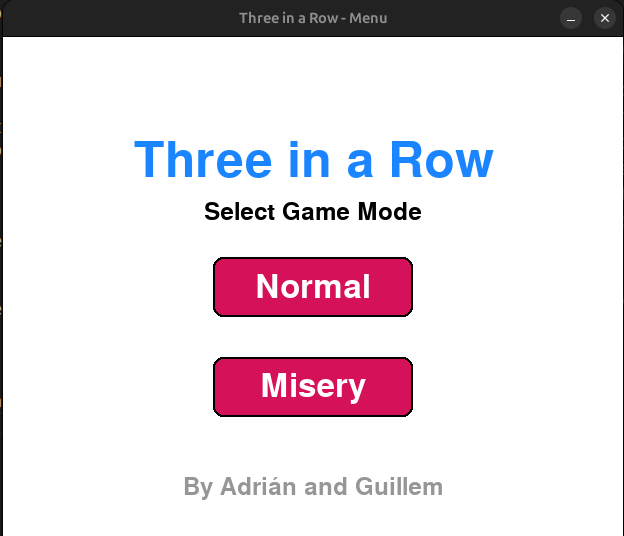
\includegraphics[scale=0.5]{./imagenes/menu_inicio.png}
    \caption{Menú principal del juego en el modo gui (Graphical User Interface).}\label{fig:men_princ1}
\end{figure}

\vspace{\baselineskip}
Dibuja una ventana con el título del juego, y con la posibilidad de seleccionar el modo de juego 'Normal' o 'Misery', con dos atractivos 
botones rojos y con un hover azul, el cual se muestra al pasar el ratón por encima, y ayuda a diferenciar el modo de juego que se va a seleccionar, además de aportar un toque
dinámico al menú. Debajo se muestran los autores del juego.
\begin{figure}[htbp]
    \centering
    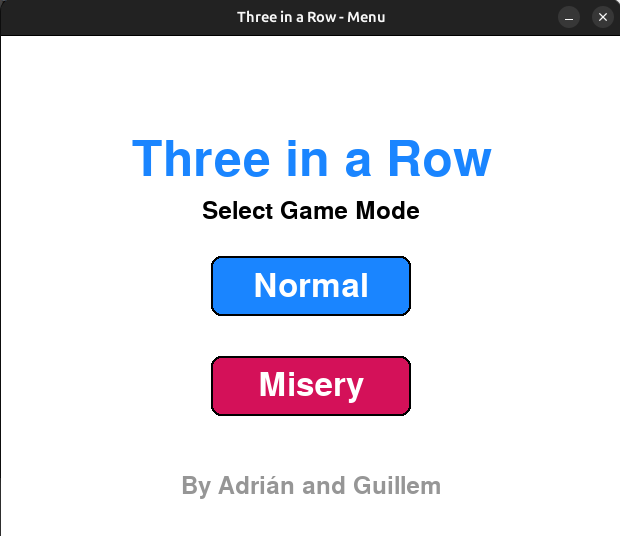
\includegraphics[scale=0.5]{./imagenes/menu_inicio2.png}
    \caption{Hover azul en el menú principal del juego.}\label{fig:men_princ2}
\end{figure}

\subsection{main\_gui.py}
Este archivo de Python es el más importante para implementar el menú del juego en modo GUI (Graphical User Interface), y el cual ofrece una interfaz de juego más amigable 
que la tradicional consola. Es sencilla de utilizar, se puede jugar con simples clicks y se visualizan correctamente todas las piedras, aunque la funcionalidad sigue siendo 
la misma que en consola. Está implementado de forma que se muestra una ventana de tamaño variable en función del tamaño del tablero, y en su fase inicial, muestra casillas 
en blanco indicando donde puede ser una piedra colocada, y un rectángulo el cual indica el color del jugador al que le toca colocar una piedra.

\vspace{\baselineskip}
\begin{figure}[ht]
    \centering
    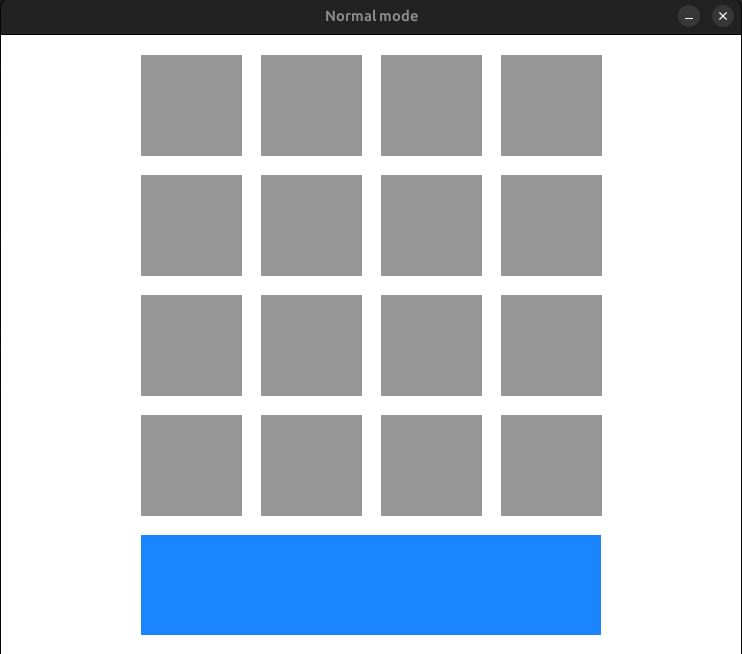
\includegraphics[scale=0.3]{./imagenes/tablero4x4.png}
    \caption{Ejemplo de tablero $4 \times 4$.}\label{fig:tablero4x4}
\end{figure}

\vspace{\baselineskip}
\begin{figure}[htbp]
    \centering
    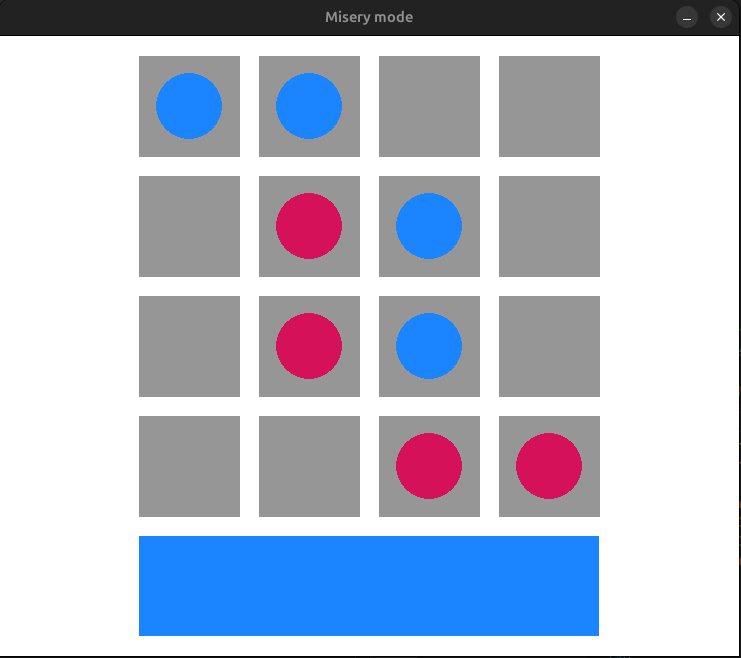
\includegraphics[scale=0.3]{./imagenes/partida4x4.png}
    \caption{Ejemplo de partida en el tablero $4 \times 4$}\label{fig:partida4x4}
\end{figure}

\vspace{\baselineskip}
Como podemos observar en la figura~\ref{fig:tablero4x4}, podemos modificar el tablero a nuestro gusto, así como las piedras de las que dispone cada jugador (para un tablero
$N \times N$, cada jugador tendrá $\frac{N^2 - 1}{2}$ piedras (siempre que $N^2 -1$ sea par)), y hacer el juego aún más interesante.

\vspace{\baselineskip}
Dentro de este archivo hemos definido varias funciones vitales para su correcto funcionamiento:
\begin{itemize}
    \item \texttt{trans\_cord}: Traduce las coordenadas de los píxeles de la ventana pygame en coordenadas del tablero.
    \item \texttt{draw\_square}: Dibuja un cuadrado en la pantalla en las coordenadas específicas del tablero, sirve para mostrar los cuadrados (tanto vacíos
    como con piedra). Se le introduce como valor el tamaño de la pantalla, y las coordenadas, y utiliza la función \texttt{pygame.draw.polygon} para conseguir esto.
    \item \texttt{draw\_stone}: Sirve para dibujar la piedra en la pantalla en las coordenadas especificadas que se le introducen a la función, así como el color en 
    función del jugador al que le toque el turno. Utiliza la misma función antes mencionada pero con un círculo (\texttt{pygame.draw.circle}).
    \item \texttt{draw\_board}: Es la función principal, y se encarg de dibujar el tablero completo, utilizando las funciones anteriormente mencionadas. Dibuja las casillas
    en horizontal y vertical, y todas las piedras que sean necesarias. Acepta el parámetro \texttt{curr\_player}, para saber cual es el jugador actual y dibujar un rectángulo 
    del color de dicho jugador, y end, para saber si debe de seguir dibujando tablero o el juego ya ha acabado.
\end{itemize}

\vspace{\baselineskip}
Para seleccionar el modo de juego, dentro de este mismo archivo, y antes de ejecutar las funciones que se encargan de ejecutar el juego propiamente dicho en el modo seleccionado,
hemos agregado una variable llamada \texttt{selected\_mode}, la cual llama a la función \texttt{show\_menu}, que invoca el menú principal del juego, y mediante los botones que se 
han mostrado anteriormente en el menú principal retorna \texttt{'normal'} si se ha seleccionado el modo normal o \texttt{'misery'}, si se ha seleccionado el modo misery.
Dependiendo del modo de juego seleccionado, se ejecuta la función correspondiente. Esto se logra mediante una estructura condicional \texttt{if} en Python.


\vspace{\baselineskip}
Posteriormente se han definido las funciones \texttt{normal\_mode} y \texttt{misery\_mode}. Hemos optado por definir dos funciones diferentes para cada modo de juego para poder 
modificar el comportamiento de cada modo de juego si fuese necesario sin que este afecte al otro, además facilitar la legibilidad del código y tener la opción de añadir nuevos 
modos de juego mucho más fácilmente.

\subsection{main\_txt.py}
El archivo \texttt{main\_txt.py} es el encargado de ejecutar el modo texto del juego 3 en raya en la consola. Este archivo contiene todas las funciones y la lógica necesarias para 
permitir a los jugadores interactuar con el juego a través de la línea de comandos. Este archivo está diseñado para ser fácil de entender y modificar sin demasiada dificultad, además
de requerir muchos menos recursos que la versión en gui.

\vspace{\baselineskip}
Se utilizan librerías como os (para ejecutar comandos de consola: limpiarla en windows y linux), y time, para añadir pausas y hacer el juego más digerible visualmente.
A continuación se explican las funciones una a una:

\begin{itemize}
    \item \texttt{clear}: Se encarga de limiar la consola en windows y linux, cambiando de comando para cada sistema operativo.
    \item \texttt{print\_header}: Imprime la cabecera del juego.
    \item \texttt{print\_turn\_indicator}: Imprime el indicador del turno del jugador.
    \item \texttt{print\_input\_prompt}: Imprime la línea donde se escribirán las coordenadas en las que el jugador quiere que se coloque cada ficha.
    \item \texttt{play\_again}: Pregunta al usuario si quiere jugar de nuevo y retorna la respuesta (True o False), la cual será utilizada posteriormente. 
    \item \texttt{spinner\_bar}: Se encarga de realizar la animación que aparece al principio del inicio del juego, no tiene ninguna funcionalidad aparte de la estética.
    \item \texttt{play\_game}: Esta función sirve para que pueda ser llamada siempre que se reinicie el juego. Dentro de ella se establecen todos los parámetros necesarios 
    para iniciar el juego, y se llama a la función \texttt{set\_board\_up} para inicializar el tablero. Dentro de esta función hay dos bucles principales:
    \begin{enumerate}
        \item Bucle para seleccionar la piedra, que utiliza \texttt{try} y \texttt{except} para capturar errores y que el juego no termine si se selecciona unas coordenadas 
        no válidas.
        \item Bucle para mover la piedra seleccionada, y al igual que antes tiene capacidad para gestionar errores eficientemente
    \end{enumerate}
\end{itemize}

\vspace{\baselineskip}
Además de todo lo anteriormente mencionado, se ejecuta un bucle principal, el cual ejecuta la función \texttt{play\_game}, y sigue ejecutándose hasta que el jugador responde que no 
desea jugar más.

\vspace{\baselineskip}
A continuación se incluyen algunas fotos del funcionamiento del juego en modo txt:

\begin{figure}[htbp]
    \centering
    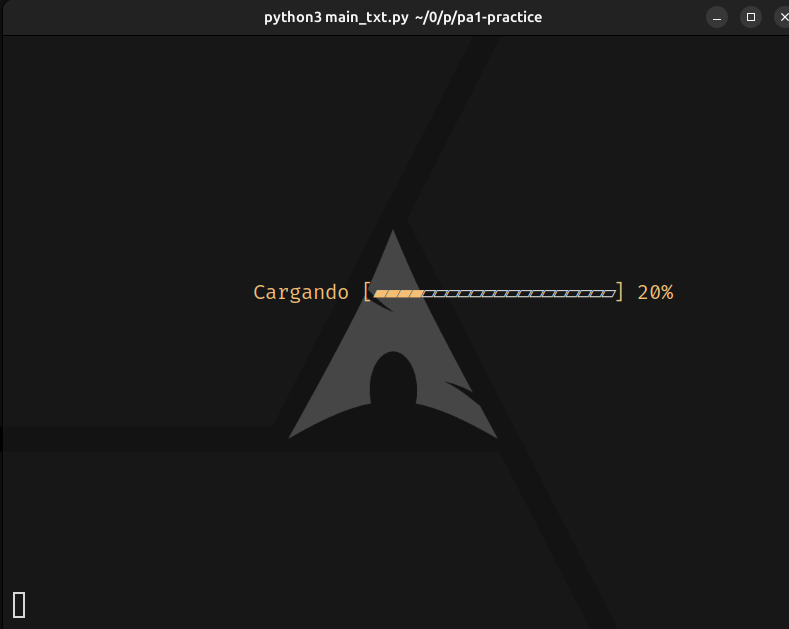
\includegraphics[scale=0.45]{./imagenes/animacion.png}
    \caption{Animación de carga.}\label{fig:animacion}
\end{figure}
\begin{figure}[htbp]
    \centering
    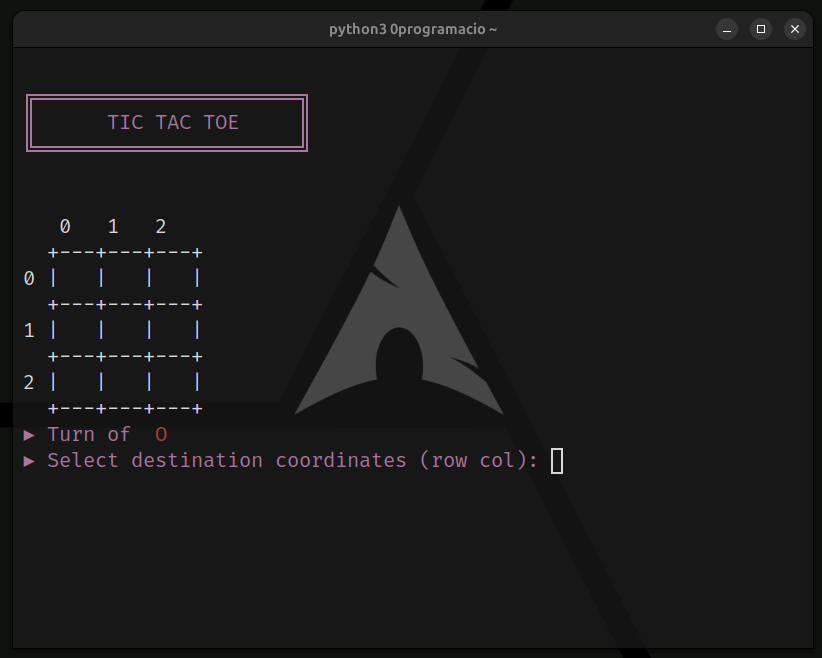
\includegraphics[scale=0.45]{./imagenes/principal_txt.png}
    \caption{Pantalla principal del juego, tablero vacío.}\label{fig:principal_txt}
\end{figure}
\begin{figure}[htbp]
    \centering
    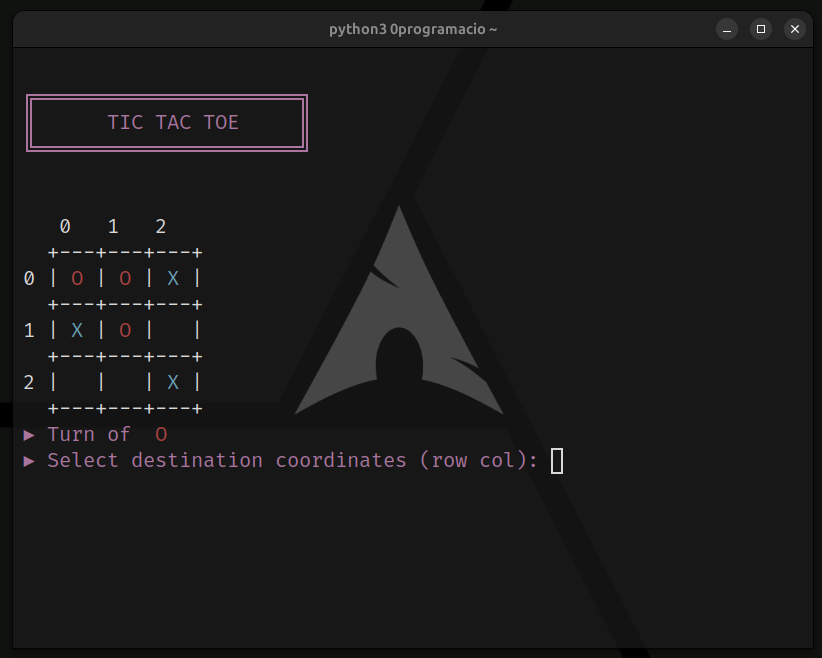
\includegraphics[scale=0.45]{./imagenes/partida.png}
    \caption{Partida a mitad de juego.}\label{fig:partida}
\end{figure}
\begin{figure}[htbp]
    \centering
    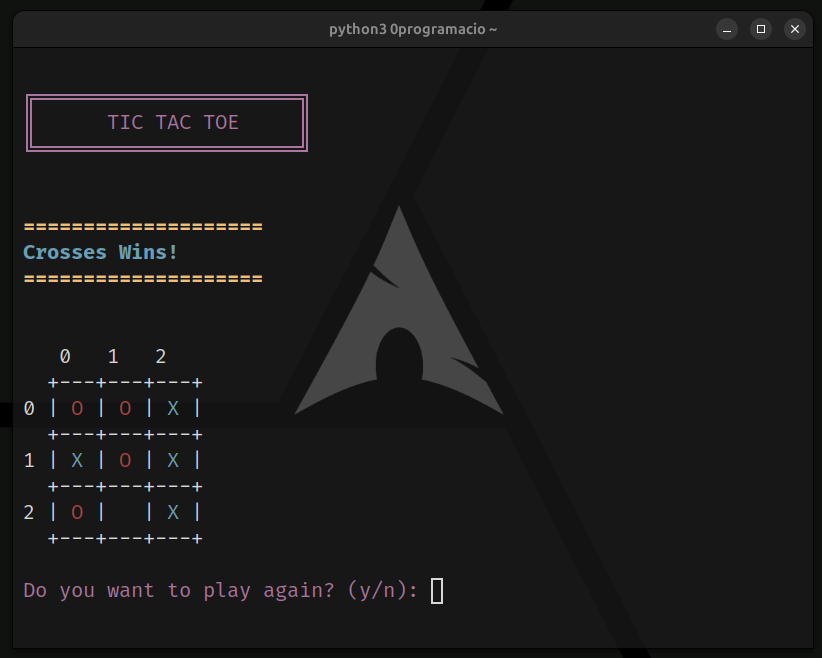
\includegraphics[scale=0.45]{./imagenes/final_partida.png}
    \caption{Final de partida, ganan las cruces (X).}\label{fig:final_partida}
\end{figure}
\newpage

\section{Bibliografía}
\begin{enumerate}
    \item \textbf{Documentación oficial de Pygame} \\
    \url{https://www.pygame.org/docs/}

    \item \textbf{Python.org} \\
    \url{https://docs.python.org/3/}

    \item \textbf{Github} \\
    \url{https://docs.github.com/es/repositories}

    \item \textbf{ASCII Art Archive} \\
    \url{https://www.asciiart.eu/}

    \item \textbf{GameDev.net} \\
    \url{https://www.gamedev.net/}

    \item \textbf{Wikipedia} \\
    \url{https://es.wikipedia.org/wiki/Tres_en_raya}

    \item \textbf{Real Python} \\
    \url{https://realpython.com/python-exceptions/}

    \item \textbf{ANSI Escape Codes} \\
    \url{https://en.wikipedia.org/wiki/ANSI_escape_code}

    \item \textbf{Python Patterns} \\
    \url{https://python-patterns.guide/}
\end{enumerate}


\end{document}

